The \textit{Notification} module is responsible for keeping the user informed 
as to when the benchmarking on their work is done. this is in place because
results will often not be instant due to factors such as queues because of server
load or algorithm needing a large of time to be throughly benchmarked. Once the
benchmarking is completed, the user will be notified by email that they can now
view their results.

\subsection{Scope}
The scope for the users module is shown in Figure \ref{Notifications Scope}
\begin{figure}[H]
	\begin{center}
		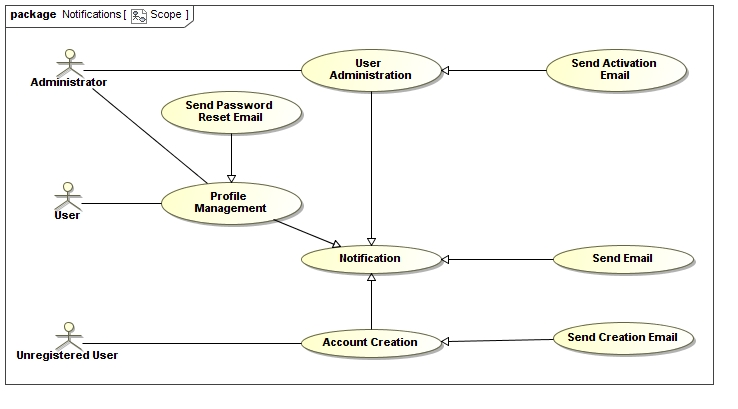
\includegraphics[scale=0.5]{../Diagrams and Charts/Notifications/Scope.jpg}
		\caption{Notifications Scope}
	\end{center}
	\label{Notifications Scope}
\end{figure}
The scope of the Notification module includes:
\begin{itemize}
	\item sendEmail
	\item sendActivationEmail
	\item sendCreationEmail
	\item sendPasswordResetMail
\end{itemize}

These use cases will be used by the User Management Module to assist with the user
authenication amoung other things. That being said the module provides the
functionality to send emails which can be used by any other module that needs this
functionality.

\subsection{Domain Model}
The domain model for the notifications module is shown in Figure \ref{Notifications Domain Model}
\begin{figure}[H]
	\begin{center}
		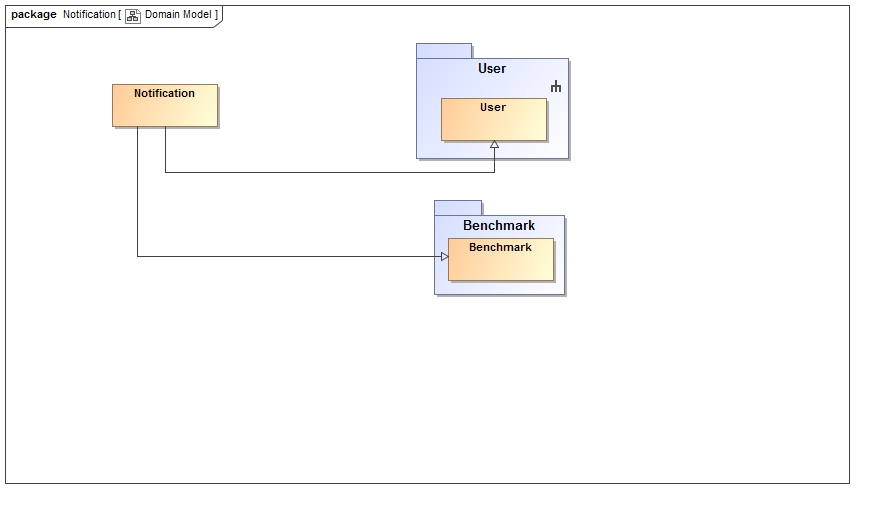
\includegraphics[scale=0.5]{../Diagrams and Charts/Notifications/Domain Model.jpg}  
		\caption{Notifications Domain Model}
	\end{center}
	\label{Notifications Domain Model}
\end{figure}

\subsection{sendEmail}
Sends an email to a spesific address with a spesified heading and content
provided all the details given are valid.

\subsubsection{Service Contract}
The service contract for the sendEmail use case is shown in Figure \ref{sendEmailServiceContract}
\begin{figure}[H]
	\begin{center}
		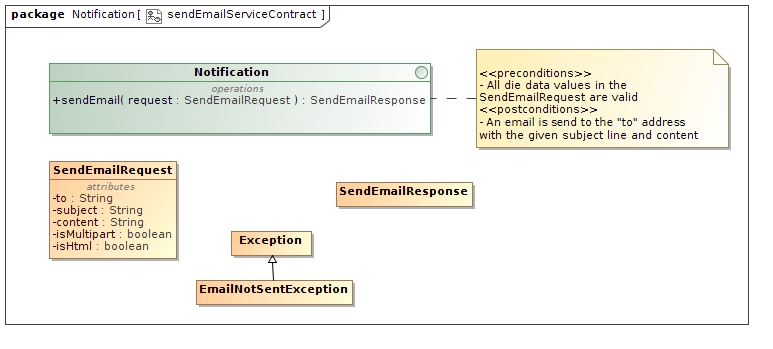
\includegraphics[scale=0.5]{../Diagrams and Charts/Notifications/sendEmailServiceContract.jpg}
		\caption{The service contract for the sendEmail use case}
	\end{center}
	\label{sendEmailServiceContract}
\end{figure}

The use case sends an email to a spesific address with a spesified heading and content
provided all the details given are valid. If any of the fields in the request object,
particularly the "to" field are not valid the serivce will throw a EmailNotSentException.

\subsection{sendActivationEmail}
Used to send a newly created managed user an email regarding the settings of
their password.

\subsubsection{Service Contract}
The service contract for the sendActivationEmail use case is shown in Figure \ref{sendActivationEmailServiceContract}
\begin{figure}[H]
	\begin{center}
		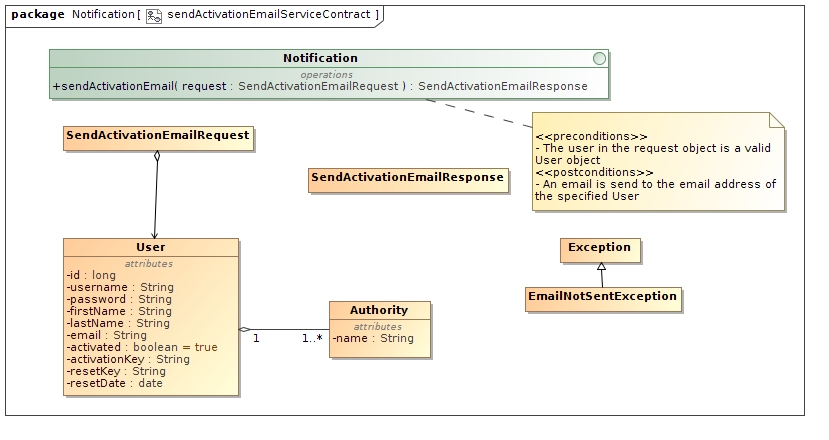
\includegraphics[scale=0.5]{../Diagrams and Charts/Notifications/sendActivationEmailServiceContract.jpg}
		\caption{The service contract for the sendActivationEmail use case}
	\end{center}
	\label{sendActivationEmailServiceContract}
\end{figure}

The use case sends an email to a spesified User. This email allows the user to
activate his account after it has been created.

\subsection{sendPasswordResetMail}
Sends an email to a specific address with a specified heading and content
with the intention resetting the users password, provided all the details 
given are valid.